\begin{frame}[parent={cmap:jabuti-software-testing},hasnext=true,hasprev=true]
\frametitle{Concepts}
\label{cmap:jabuti-gui}
\label{cmap:graphical-user-interface}
\label{cmap:gui}

\insertcmap{Courses-SoftwareTesting-JaBUTi-JaBUTiUserInterfaceGraphical}
\end{frame}


\begin{frame}[parent={cmap:jabuti-gui},hasnext=true,hasprev=true]
\frametitle{Graphical user interface (GUI)}
\label{concept:jabuti-gui}

\begin{block}{JaBUTi GUI}
\begin{itemize}
	\item Allows the beginner to explore and learn the concepts of
	control-flow and data-flow testing.

	\item Provides a better way to visualize which part of the classes
	under testing are covered and which are not.
\end{itemize}
\end{block}

\begin{block}{Demo}
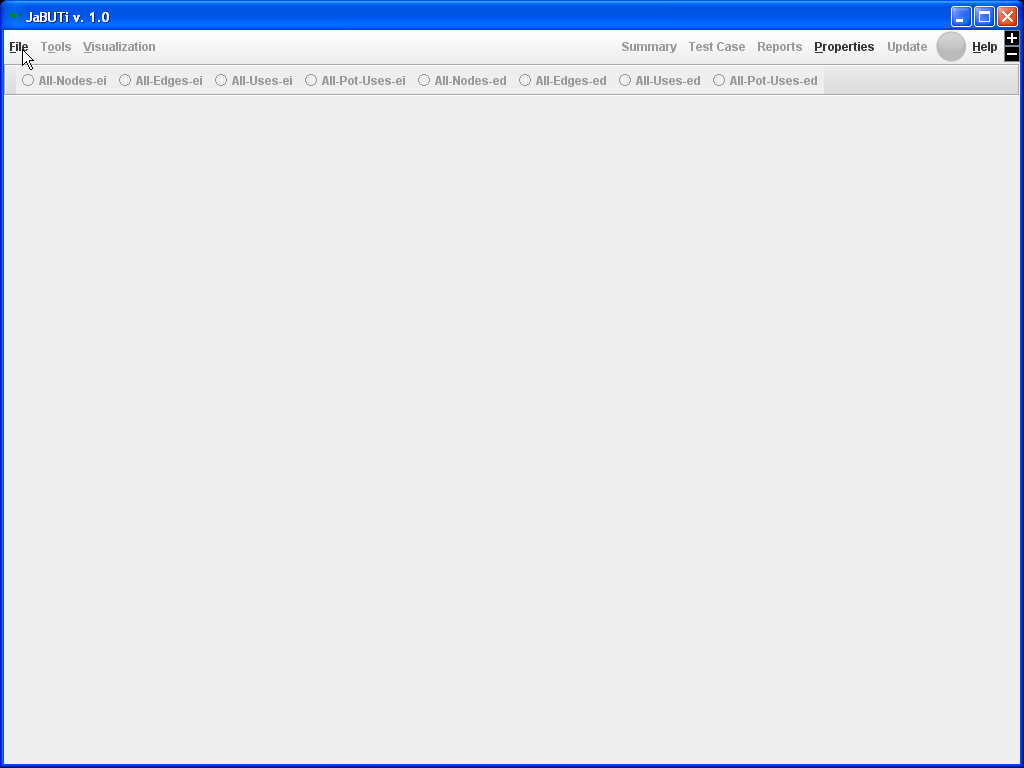
\includegraphics[width=\textwidth,clip]{resources/JaBUTi/JaBUTi-GUI/JaBUTi-GUI}
\end{block}
\end{frame}


\begin{frame}[c]
\frametitle{Graphical user interface}
\framesubtitle{Main functionalities}
\label{concept:main-functionalities}

\vfill
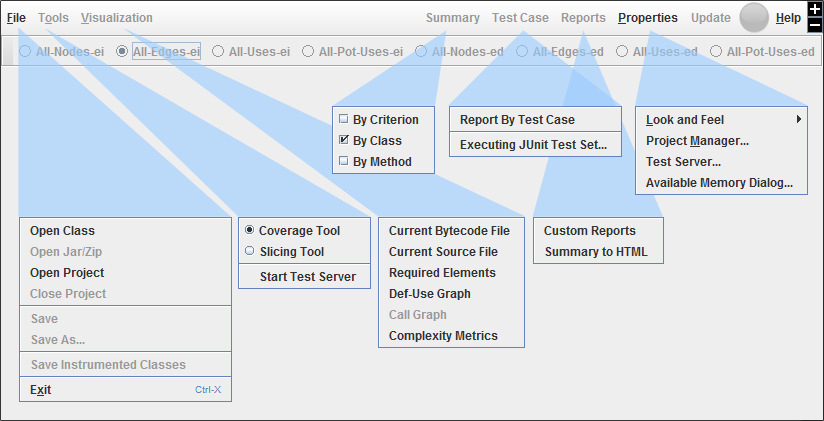
\includegraphics[width=\textwidth,clip]{resources/JaBUTi/JaBUTi-GUI/JaBUTi-GUI-Expanded}
\vfill
\hfill
\refie{example:jabuti-gui-demo}{\beamerbutton{Demonstration of JaBUTi capatibilities}}
\end{frame}

